%%This is a very basic article template.
%%There is just one section and two subsections.
\documentclass{template/llncs}

%\usepackage{lineno}
\usepackage{amssymb}
\usepackage{graphicx}
% declare the path(s) where your graphic files are
\graphicspath{{./pictures/}}
% and their extensions so you won't have to specify these with
% every instance of \includegraphics
\DeclareGraphicsExtensions{.pdf}
\usepackage{color}

% Needed for next-to-each-other figures
\usepackage{subfig} 

% Needed for top and bottom rules
\usepackage{booktabs}

% Needed for text rotation in tables
\usepackage{rotating} 
 
% Needed for lightning symbol
\usepackage{wasysym}

% Needed for striking out text or formula from bottom left to top right
\usepackage{cancel}

\usepackage{upgreek}

\usepackage{pgfplots}
 
\usepackage{multirow}
\usepackage{url}
% enables to use rotated text (defined in package 'rotating') in rows of tables defined in command 'tabular::multicolumn' 
\usepackage{array}
\newcolumntype{v}[2]{%
  >{\begin{turn}{#1}\begin{minipage}{#2}\raggedright\hspace{0pt}}l%
  <{\end{minipage}\end{turn}}%
}

\usepackage{enumitem}

\usepackage{listings}  % um Code-Fragmente darzustellen

% dotted lightning (to be used within math-environments)
\newcommand*{\dotlightning}[0]{\cdot$\lightning$\cdot}
% alternate symbol of dotted lightning (to be used within math-environments)
\newcommand*{\dotlightningAlt}[0]{\cdot$f$\cdot}
% dotted x (to be used within math-environments)
\newcommand*{\dotx}[0]{\dot{\times}}

\newcommand{\dotl}[0]{\lessdot}
\newcommand{\dotg}[0]{\gtrdot}
\newcommand{\triple}[3]{#1_S \stackrel{#2}{\leftarrow} #1_C \stackrel{#3}{\rightarrow} #1_T}
\newcommand{\TGG}[0]{\mathcal{L}(TGG)}

\newcommand{\stereotype}[1]{{\small$\ll$}#1{\small$\gg$}}

\newcommand{\TODO}[1]{\textcolor{red}{TODO: #1}}
% data structure 
\renewcommand{\O}[0]{{\Upomega}}

% precedence function
\newcommand{\PF}[0]{\mathcal{PF}}

% precedence sequence
\newcommand{\PS}[1]{\mathcal{PS}(#1)}
\newcommand{\PSp}[2]{{#2}(\PS{#1})}

\hyphenation{Spe-ci-fi-ca-tions e-mer-ging}

\begin{document}

\mainmatter
\title{Model-based Generation of Run-time Monitors for AUTOSAR}
\author{Lars Patzina\inst{1}%
\and Sven Patzina\inst{1}
\and Thorsten Piper\inst{2}
\and Paul Manns\inst{2}}

\institute{Real-Time Systems Lab, Technische Universit\"{a}t Darmstadt, Darmstadt, Germany\\
\email{\{sven.patzina, lars.patzina\}@es.tu-darmstadt.de}
\and
DEEDS Group, Technische Universit\"{a}t Darmstadt, Darmstadt, Germany\\
\email{\{piper, manns\}@cs.tu-darmstadt.de}}

\maketitle

%\begin{linenumbers}

\begin{abstract}
Driven by technical innovation, embedded systems, especially in vehicles, are becoming increasingly interconnected and, consequently, have to be secured against failures and threats from the outside world.
One approach to improve the fault tolerance and resilience of a system is run-time monitoring.
AUTOSAR, the emerging standard for automotive software systems, specifies several run-time monitoring mechanisms at the watchdog and OS level that are neither intended, nor able to support complex run-time monitoring.
This paper addresses the general challenges involved in the development and integration of a model-based generation process of complex run-time security and safety monitors.
A previously published model-based development process for run-time monitors based on a special kind of Petri nets is enhanced and tailored to fit seamlessly into the AUTOSAR development process.
In our evaluation, we show that efficient monitors for AUTOSAR can be directly modeled and generated from the corresponding AUTOSAR system model.
    

%Defining a complete monitor specification with this language is a very complex task, because every LSC stands for its own and has to define its preconditions itself.
 
%Furthermore, the generated monitor based on the specification monitors every signature described as LSC all the time, which leads to a not acceptable run-time behavior. 
 
\keywords{AUTOSAR, extended live sequence charts, model-based, monitor petri nets, run-time monitoring, signatures }
\end{abstract}

%Intro
\section{Introduction}\label{sec:introduction}

Embedded systems are becoming increasingly interconnected and can no longer be considered as being separated from the outside world. 
A prominent example are multimedia systems in the automotive domain that are connected to the internet without being totally separated from safety-critical components.
Many systems have been developed as closed systems and often little attention has been paid to security mechanisms such as encryption and safe component design to deal with errors and attacks. 
Even modern networks in the automotive domain are vulnerable to passive and active attacks \cite{Groll2009} and protocols such as the CAN bus protocol have been identified as a major security drawback \cite{Koscher2010}.
This makes it necessary to secure safety-critical components and their communication, even if they are not directly accessible. 
To secure these systems, Papadimitratos et al. \cite{Papadimitratos2008} propose a secured communication and demand a secure architecture.
However, in the majority of cases, even such efforts cannot eliminate all security vulnerabilities that can lead to safety threats as it is impossible to foresee all attacks during development. 
Moreover, it is often economically or technically infeasible to secure existing systems retroactively against external adversaries.
Hence, systems and especially electronic control units in cars cannot be considered as secure against attacks, either caused by unknown vulnerabilities or by the required integration of legacy components. 
To cope with these security and safety issues, run-time monitoring is a feasible approach to detect attacks that exploit previously unknown errors and security vulnerabilities \cite{Kumar1995}.

The AUTOSAR (AUTomotive Open System ARchitecture) platform\footnote{AUTOSAR: http://www.autosar.org} is emerging in the automotive domain as an open industry standard for the development of in-vehicular systems.
To cope with the growing complexity of modern vehicular systems, it provides a modular software architecture with standardized interfaces and a run-time environment (RTE) that separates application level software components from the underlying basic software modules and the actual hardware.  
AUTOSAR offers a clearly structured system specification, which is stored in the standardized AUTOSAR XML (ARXML) format. 
The AUTOSAR development process supports the monitoring of control flow and timing properties at a low abstraction level~\cite{AUTOSAR_OS_SPEC,AUTOSAR_WDM_SPEC}, but does not provide support for modeling complex monitoring functionality at the software component level.

For this purpose, we have adopted our generic Model-based Security/Safety Monitor (MBSecMon) development tool chain~\cite{Patzina2011}. 
It is based on the Model-Driven Development (MDD) concept that supports the generation of monitors from signatures describing the interactions between the components of a system.
The MBSecMon specification language (MBSecMonSL) is based on Live Sequence Charts (LSC) introduced by Damm and Harel~\cite{Damm2001}, which have been extended \cite{Patzina2011} for the modeling of behavioral signatures.
A specification based on these extended LSCs (eLSC) and a structural description of the system constitutes the input set of the MBSecMon process. 
The signatures are divided in intended system behavior (use cases) and known attack patterns and attack classes (misuse cases). 
These signatures are automatically transformed to a formally defined Petri net language, the Monitor Petri nets (MPNs) \cite{Patzina2010}, which serve as a more explicit, intermediate representation.
With the provision of platform-specific information, security/safety run-time monitors are automatically generated for different target platforms.
%\textcolor{red}{Target platforms supported are C, Java, VHDL \ldots}
%\textcolor{red}{Monitors can be fed with information by wrappers around the AUTOSAR components, instrumentation framework\cite{Piper2012}}

The contribution of this paper is the development of a methodology for the model-based development of complex run-time monitors for AUTOSAR that operate directly on the AUTOSAR system model.
%address the lack of complex run-time monitoring support in AUTOSAR tool chains.
We depict the challenges that arise during the development and integration of a model-based monitor generation framework into the AUTOSAR development process and present solutions to each.
In summary, these challenges are as follows.
\begin{enumerate}[label=\textbf{C\arabic{enumi}},ref=\arabic{enumi}]
  \item \label{itm:integrationExisting} Integrating existing AUTOSAR development fragments into the monitor generation process. 
  \item \label{itm:datatypesafety} Providing type safety during the whole modeling and generation process of the monitors.
  \item \label{itm:modelling} Modeling monitor signatures on the same abstraction level as the AUTOSAR system models.  
  \item \label{itm:mappingsig} Mapping of the abstract signature descriptions to platform specific monitoring code.
  \item \label{itm:connectingmonitors} Providing communication data of the generated AUTOSAR software components (SW-C) to the monitors. 
  \item \label{itm:relocatability} Supporting the relocatability of software components by generating distributed monitors from global signatures.
  \item \label{itm:minimalOverhead} Generating monitors with a minimal overhead for the control units. 
\end{enumerate}

% \begin{itemize}
%   \item Model-based approach for monitor specification and generation incorporating existing AUTOSAR specifications independent from the used AUTOSAR tool chain
%   \item Using the AUTOSAR XML system view for modeling signatures
%   \item Usage of existing development artifacts such as sequence charts that can be extracted from existing specification documents or traces
%   \item Automatic generation and integration of complex monitors in AUTOSAR generated code via automatic minimal instrumentation of the application code.
% \end{itemize}

%\textcolor{red}{restriction to data-oriented Sender-Receiver Interface?}

The remainder of the paper is structured as follows: 
Section~\ref{sec:relatedWork} gives an overview of existing approaches for monitoring and instrumentation and describes how they can be applied in the AUTOSAR process.
In Sect.~\ref{sec:mbsecmonFramework}, the challenges are described in detail, and solutions are presented based on the adaptation of the MBSecMon process for the AUTOSAR development process.
%After that, the mentioned challenges are described in detail and solutions based on adaption of the MBSecMon process to the AUTOSAR development process are shown in Section~\ref{sec:mbsecmonFramework} by using an example from the automotive domain.
The generated monitors that are connected to the example system are evaluated in Sect.~\ref{sec:evaluation}.
In Sect.~\ref{sec:conclusion}, a conclusion is drawn, and possible future work is discussed.


\section{Related Work}
\label{sec:relatedWork}

The AUTOSAR standard specifies several run-time monitoring mechanisms that are provided by the Operating System (OS) and the Watchdog Manager (WdM).
In the \emph{Specification of Operating System} \cite{AUTOSAR_OS_SPEC}, three monitoring mechanisms for the detection of timing faults at run-time, i.e., tasks or interrupts missing their deadline, are considered.
\emph{Execution time protection} monitors the execution budget of tasks and category 2 Interrupt Service Routines (ISRs), in order to guarantee that the execution time does not exceed a statically configured upper bound.
\emph{Locking time protection} supervises the time that a task or category 2 ISR can hold a resource, including the suspension time of OS interrupts or all interrupts of the system.
This is done to prevent priority inversions and to recover from potential deadlocks.
The third monitoring mechanism is \emph{inter-arrival time protection}, which controls the time between successive activations of tasks and the arrival of category 2 ISRs.
These mechanisms monitor the system at the task level and are not suited to implement control flow or data flow monitoring.
The configuration is done at the OS level and does not factor the system view of the model.

The \emph{Specification of Watchdog Manager} \cite{AUTOSAR_WDM_SPEC} provides three monitoring mechanisms that are complementary to those offered by the AUTOSAR OS.
All of the implemented mechanisms are based on checkpoints that report to the watchdog manager (WdM) when they are reached.
Supervised functions have to be instrumented with calls to the watchdog, which verifies at run-time the correct transition between two checkpoints as well as the timing of the checkpoint transitions.
For \emph{alive supervision}, the WdM periodically checks if the checkpoints of a supervised entity have been reached within the given limits, in order to detect if a supervised entity is run too frequently or too rarely.
For the supervision of aperiodic or episodical events that have individual constraints on the timing between checkpoints, the WdM offers \emph{deadline supervision}.
In this approach, the WdM checks if the execution time of a given block of a supervised entity is within the configured minimum and maximum bound.
The third mechanism that the WdM provides is \emph{logical monitoring}, which focuses on the detection of control flow errors, which occur if one or more program instructions are processed either in an incorrect sequence or are not processed at all.
This approach resembles the work of Oh et al. \cite{Oh2002}, in which a graph representation of a function is constructed by dividing the function into \emph{basic blocks} at each (conditional) branch.
Basic blocks are represented by nodes, whereas legal branches are represented by arcs that connect the nodes. 
Whenever a new basic block is entered, the monitor verifies that the taken branch was legal, according to the graph representation.

Except for control flow monitoring, the monitoring mechanisms that AUTOSAR currently specifies are only suitable for monitoring timing properties at a low level of abstraction. 
None of the approaches is configured on the level of the AUTOSAR system model, which offers the developer an intuitive and integrated view on the system.
Apart from the monitoring services offered by AUTOSAR, few research has covered this area so far.
One exception are two articles by Cotard et al. \cite{Cotard2012a,Cotard2012b}, in which the authors describe a monitoring approach for the synchronization of tasks on multi-core hardware platforms. 
In their approach, dependencies between tasks are first modeled as a finite state machine (FSM).
The FSM is then translated into a linear temporal logic (LTL) specification, from which Moore machines and, subsequently, C code is generated.
Their primary focus is on synchronization and not on control or data flow monitoring.
%Today, in industry mostly hand programmed watchdog monitors are used that are programmed directly in the target language (C).
%This allows individual monitors for every purpose, but is not well integrated into the AUTOSAR process.
%Conventions, such as naming conventions of AUTOSAR, have to be kept by the programmer and errors in the monitoring code are possible.
%
%To reduce the risk of errors in monitors a model-based specification eases the modeling for the programmer, and the specification gets more readable.
%There are different modeling languages for signatures that can be used for communication and program flow monitoring. 
%EDL~\cite{Schmerl2006}, 
%simple PN languages for monitors in embedded systems~\cite{Frankowiak2009} 
%These languages are only usable for small monitor definitions.
%A framework that is similar to our MBSecMon process is the Monitoring Oriented Programming framework (MOP) \cite{Meredith2011}. Is based on Java.
%
%Are they integrated in the AUTOSAR development Process?

%Support of (Windowed) Watchdog Concept\footnote{http://www.autosar.org/download/R2.0/AUTOSAR\_SWS\_WatchdogManager.pdf}?
%\begin{itemize}
%\item Watchdog manager located n Basic Software, uses hardware watchdog timers over the drivers and accesses the software components via RTE.
%\item allows for alive supervision of single or multiple sw-components (sw-component proves aliveness by updating counter) and non-alive supervision (manager triggers periodically the sw-components)
%\end{itemize}  
%
%Communication Watchdog for periodic messages~\cite{AUTOSAR2011}\\\\
%
%\begin{description}
%  \item[!] Program Flow Monitoring
%  \item[?] Modeling with LSCs (maybe in Section~\ref{sec:mbsecmonFramework})
%  \item[?] Code Generation (maybe in Section~\ref{sec:mbsecmonFramework})
%  \item[?] Instrumentation
%\end{description}

% Another approach is ... TODO: enter healing paper here - The paper "A framework for health monitoring of automotive electrical and electronic control systems" does explicitely not address AUTOSAR. Therefore not really well suited as related work.


% In our process, the expressive and compact Live Sequence Chart descriptions are transformed to a more explicit representation of their semantics represented as Monitor Petri nets.
% These are then used for code generation.
% Mostly, transformations from different source models to Petri nets and temporal logics are performed to analyze and verify the correctness of the source model.
% Amorim et al. \cite{Amorim2006} has defined a transformation from LSC to Colored Petri nets (CPN) to analyze the LSC definitions by simulating the CPNs.
% Fernandez et al. \cite{Fernandes2007} transforms use cases that are specified by sequence diagrams (SD) to CPN with the goal to obtain an executable model that is easier to understand than SDs.
% Therefore, his approach makes extensive use of the ML language, a functional programming language, and hierarchical structures to get ``readable'' results.
In our MBSecMon process, an extended version of the expressive and compact Live Sequence Charts is used as signature specification language. 
Kumar et al. \cite{Kumar2009} specifies protocols with LSCs and transforms them for verification to temporal logic formulas. 
Thereby, complex LSC specifications lead to an explosion of the formula and are, therefore, with LSCs as specification language not suitable as intermediate language for the code generation for embedded systems.

Besides these transformations to LTL, there are some approaches that use Petri nets directly for the specification of monitors.
Frankowiak et al. \cite{Frankowiak2009} uses Petri nets to specify low cost process monitors on a micro controller.
He enhances regular Petri nets by token generators and special end places (bins).
Additionally, subnets are linked by a control net.
For complex monitor specifications, these nets get relatively large compared to MPNs, whose semantics include an implicit evaluation logic when an event does not match to the specified sequence. 
The MPNs are tailored to describe monitor specifications in an explicit but nevertheless compact form.

%``A Dataflow Monitoring Service Based on Runtime Verification for AUTOSAR OS: Implementation and Performances''~
%\begin{itemize}
%  \item based on manual specified FSM, translated in LTL specification, generates Moore machines and then C code( mapping of system model and Moore machines), focused on temporal aspects
%  \item domain specific (no instrumentation (of SW-Cs, but the RTOS kernel)) plugged into RTOS kernel
%  \item each send and receive operation is intercepted and forwarded to a monitoring service
%\end{itemize}
%We:
%\begin{itemize}
%  \item higher abstraction level for modelling
%  \item Monitor at software component level
%  \item only necessary events are intercepted by instrumentation
%\end{itemize}


\section{The MBSecMon Framework}\label{sec:mbsecmonFramework}
The Model-based Security/Safety Monitor (MBSecMon) Framework~\cite{Patzina2011} has been developed as a generic approach to build tool chains for monitor generation.
In this section, we show how this framework has been tailored to fit seamlessly in a model-based AUTOSAR development process and solve the challenges that are raised in Sect.~\ref{sec:introduction}.
This overcomes the current lack of model-based monitoring support in AUTOSAR tool chains that we attested in Sect.~\ref{sec:relatedWork}.
%To cope with the high degree of abstraction between the model and the implementation an instrumentation tool~\cite{Piper2012} for AUTOSAR specifications is used.

\subsection{Example: Automatic Transmission Controller}\label{sec:example}
The example used throughout this paper focuses on monitoring the communication between AUTOSAR software components (SW-Cs). %, despite the MBSecMon framework is not limited to this application scenario.
The AUTOSAR system is modeled with the tool OptXware Embedded Architect\footnote{OptXware: http://www.optxware.com} and the implementation of the subsystems is generated by the AUTOSAR code generation of MathWork's Embedded Coder plugin for Simulink.
 
The implementation of the example system is based on the \emph{Automatic Transition Controller} demo project~\cite{TheMathWorks2012}, shipped with Matlab/Simulink.
As depicted in the system model in Fig.~\ref{fig:simulinkExample}, this model describes the internal behavior of three application-level software components, \emph{ShiftLogic}, \emph{Transmission}, and \emph{Engine}, based on the input values \emph{Throttle} and \emph{BrakeTorque} and the interaction between these components.
Influences such as aerodynamics and drag friction of the wheels are represented by the \emph{Vehicle} block.    
%As source for an realistic but not too complicated example model, depicted in Fig.~\ref{fig:simulinkExample}, the Automatic Transmission Demo project of Matlab/Simulink is used.
To comply with the needs of the AUTOSAR code generation provided by Embedded Coder, the behavioral model has been adapted by replacing all continuous with discrete blocks.
The generated code serves as the behavioral implementation of the skeleton generated by the AUTOSAR tool OptXware Embedded Architect.    
\begin{figure}[tb]
\begin{center}
  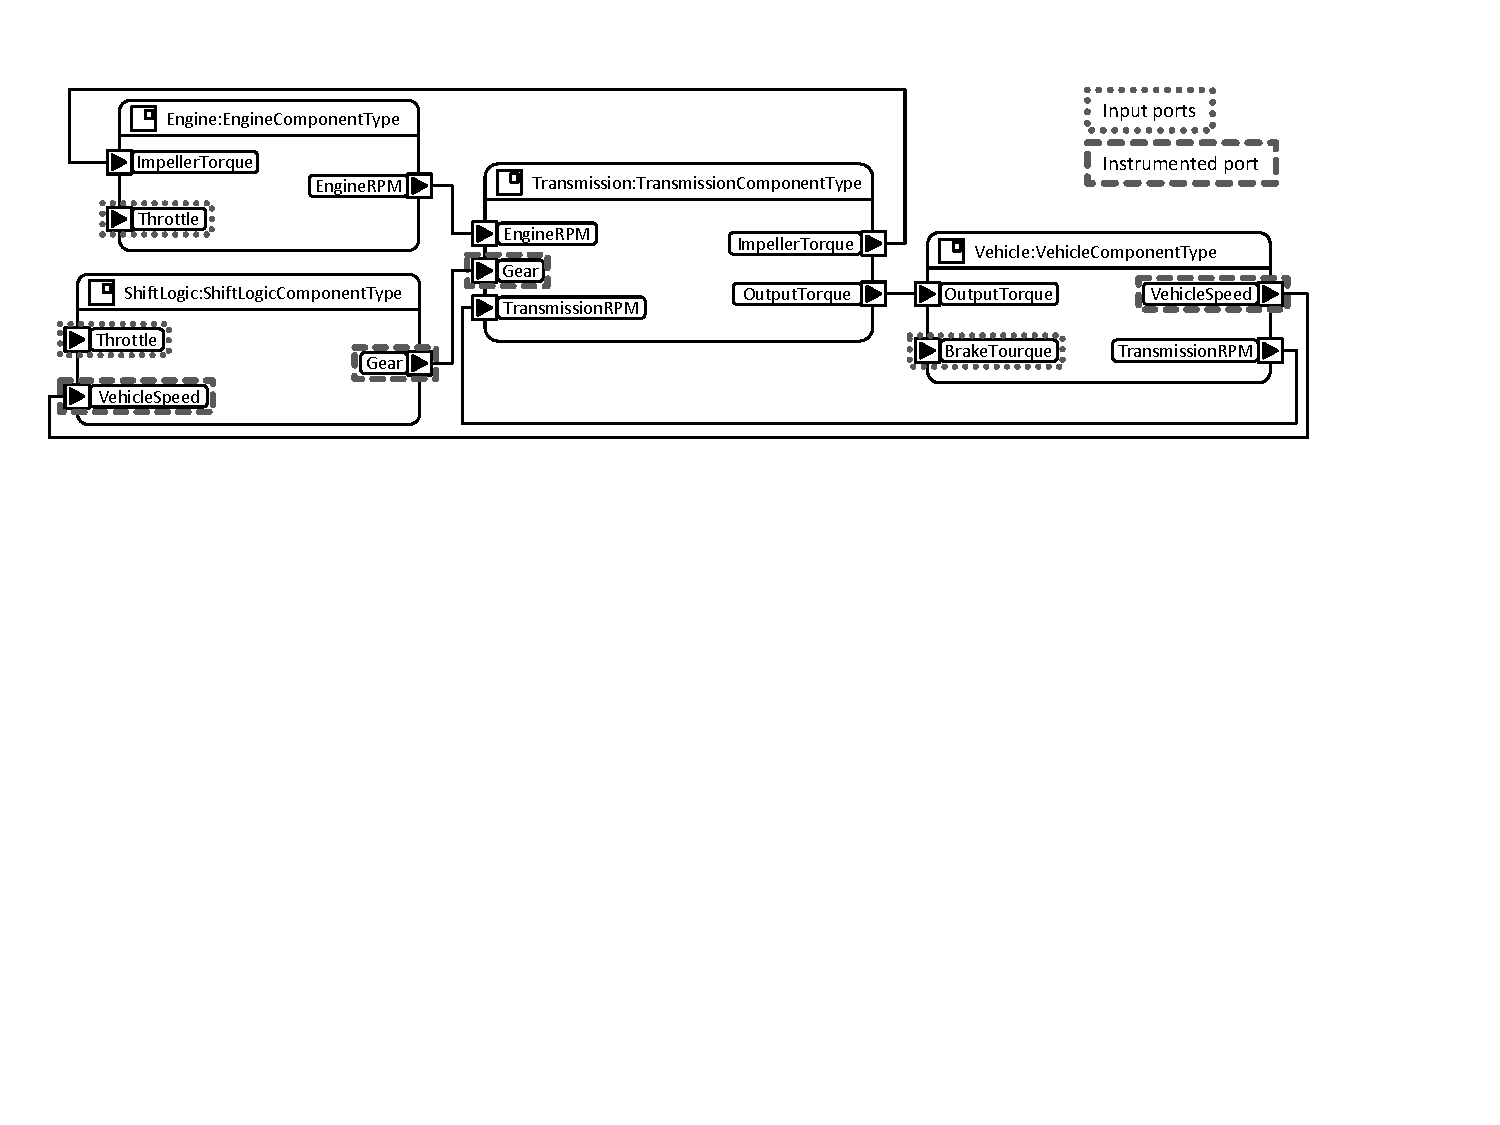
\includegraphics[width=1\textwidth]{AutomaticTransmission.pdf}
  \caption{AUTOSAR example model of an automatic transmission}
  \label{fig:simulinkExample}
\end{center}
\end{figure}
For the asynchronous communication between the components, the sender-receiver communication pattern is used.
%, where the sender does not know the identity and the number of the receivers.
%This pattern is intended to support the transferability of software components.
%auskommentiert, da die transferability/code reuse durch den VFB gew�hrleistet wird, nicht so sehr durch sender/receiver pattern
%The system consists of three components and one component that simulates the behavior of the vehicle.
%As external inputs the throttle and the brake torque are fed into the system and the outputs are throttle, engine RPM and the vehicle speed.
 
%Modeling of component structure and communication channels in OptXware Embedded Architect
%system and implementation from MATLAB model by separation of components and integration into AUTOSAR simulation code 
%- scheduling?

\subsection{The Tailored Monitor Generation Process for AUTOSAR}
%Explanation of the tailored MBSecMon Process in Fig.~\ref{fig:mbsecmonProcess}.
%\usepackage{graphics} is needed for \includegraphics
\begin{figure}[tb]
\begin{center}
  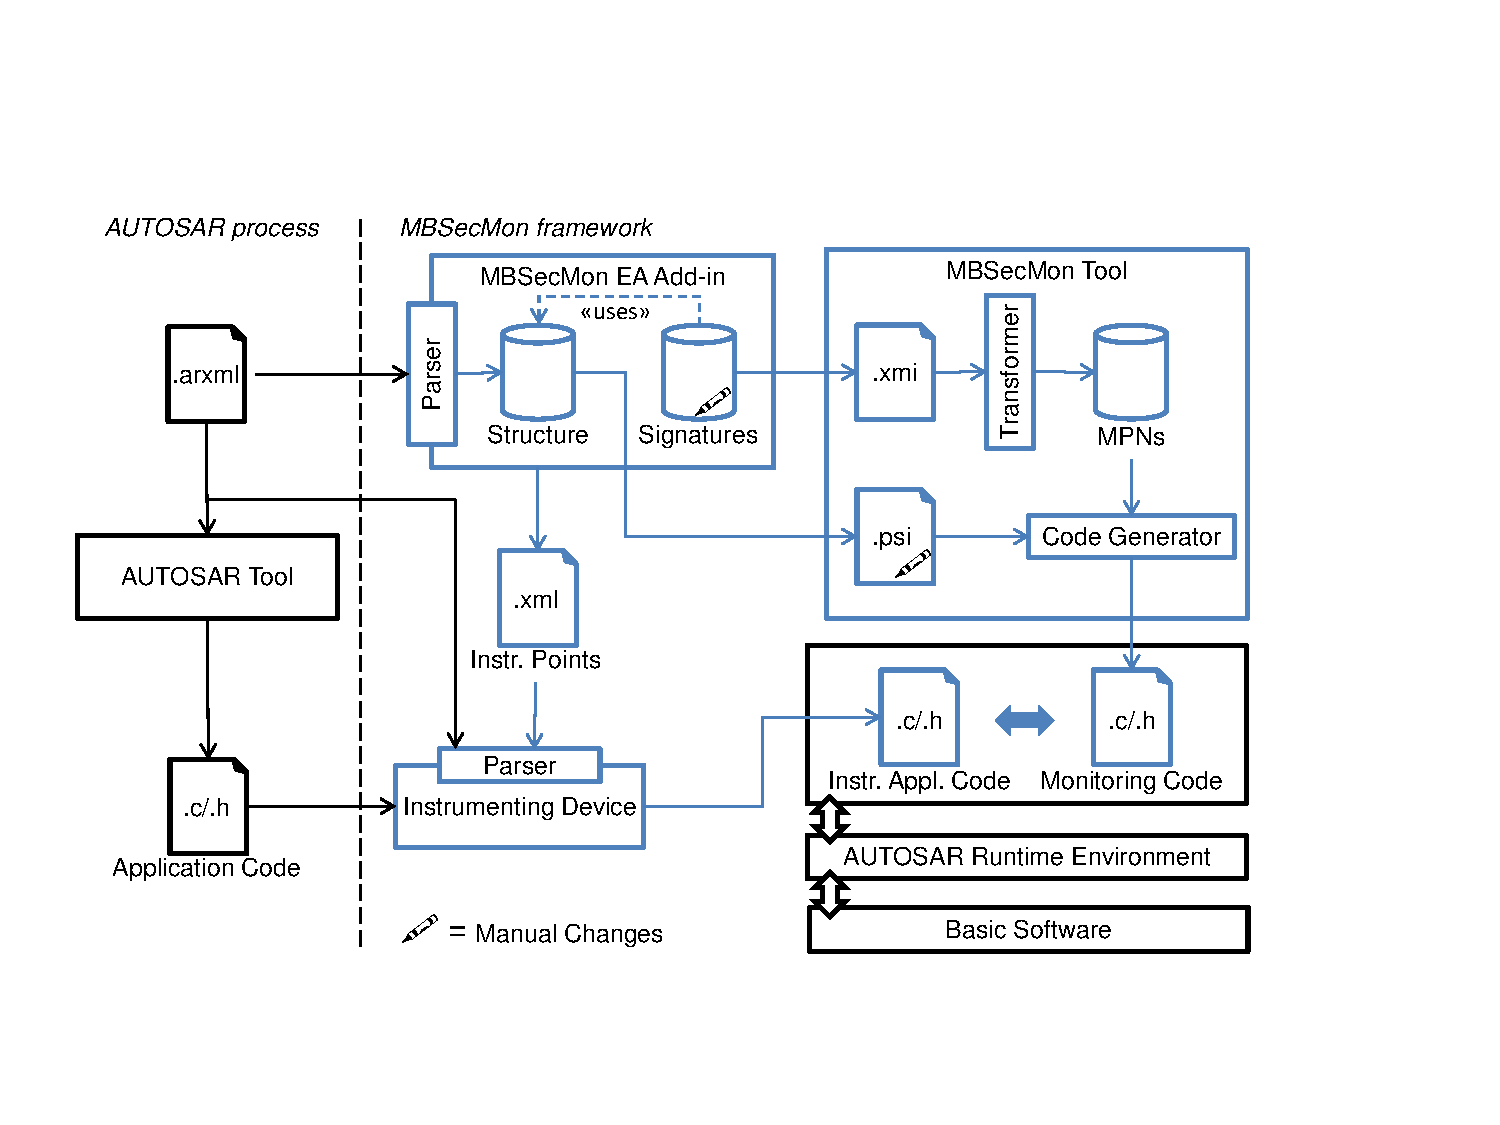
\includegraphics[width=0.75\textwidth]{MBSecMonProcess}
  \caption{MBSecMon framework embedded in AUTOSAR development process}
  \label{fig:mbsecmonProcess}
\end{center}
\end{figure}
The generic MBSecMon development tool chain has been extended to enable a seamless integration into the AUTOSAR development process.    
Figure~\ref{fig:mbsecmonProcess} depicts on the left side the original simplified AUTOSAR development process, starting with the system structure description persisted in the AUTOSAR XML format (ARXML).
This file is used by the AUTOSAR tool chain to generate the RTE and a code skeleton for the implementation of the SW-Cs, which  is supplied by the Simulink code generator. The final code is usable in an AUTOSAR simulation environment or directly on the Electronic Control Unit (ECU) of a vehicle.

On the right-hand side of Fig.~\ref{fig:mbsecmonProcess}, the framework is depicted that embeds the monitor generation tool chain in the AUTOSAR development process.
%As source documents an ARXML file that describes the component view of the system exists.
%At first, we will give an overview of the process for generating monitors.
The specification of monitor signatures is achieved with the help of a tailored version of the UML2 modeling tool Enterprise Architect\footnote{SparxSystems Enterprise Architect: http://www.sparxsystems.com} (EA).
This tool has been extended by an add-in that allows the modeling of eLSCs (\emph{Signatures}) depending on the imported component diagram view (\emph{Structure}) of the AUTOSAR system.% that has been persisted as an ARXML file.
%The structure of the AUTOSAR system is imported from the ARXML file into Enterprise Architect.
%Based on the imported component view of the model \emph{signatures} described by eLSCs are modeled.
The modeled signatures are then exported together with additional platform specific information (PSI) extracted from the imported AUTOSAR model.
Additionally, the \emph{MBSecMon add-in} analyses the modeled signatures for needed \emph{instrumentation points} in the AUTOSAR application code and persists this information in an XML file. 
Through a graph-based model-to-model transformation~\cite{Patzina2012}, the exported representations of the signatures are transformed in the formally defined Monitor Petri nets (MPNs)~\cite{Patzina2010} that serve as an intermediate language used for a straight-forward code generation.
The code generator translates the signatures, represented as MPNs, incorporating the additional information (PSI), to monitoring code.
This monitor is stimulated by calls of its interfaces. 
Therefore, the \emph{instrumenting device} uses the AUTOSAR system specification, together with the \emph{instrumentation points} file, to instrument the application code.
The instrumentation is realized via interface wrappers, which intercept the communication between two components.
A detailed description of the instrumentation of the interfaces of AUTOSAR components with wrappers is given in~\cite{Piper2012}.

This process allows for specifying and automatically generating monitors on an abstract level based on the system information provided by the AUTOSAR development process. 
Only the specification for the monitors has to be modeled using the MBSecMon add-in and the platform specific information has to be extended by the system engineer.   
In the following, based on the example in Sect.~\ref{sec:example}, this process and the necessary adaptation based on the identified challenges are described in detail. 
% Extensions for AUTOSAR
% \begin{itemize}
%   \item import for component diagrams from ARXML
%   \item restriction of modeling freedom, based in imported information
%   \item extension of exported PSI-File for code generation
%   \item export information for instrumentation 
%   \item code generation
%   \begin{itemize}
%     \item type safe AUTOSAR conform interfaces
%     \item translation of external AUTOSAR events to internal monitor events
%  \end{itemize}
% \end{itemize}

\subsubsection{Challenge \ref{itm:integrationExisting}: Integrating existing development fragments.}%$~~$\\
In the AUTOSAR development process, the system structure is modeled at a high abstraction level, describing the  software components (SW-C), their ports with specified data types, and the connections between the ports. 
The generated monitors should observe the communication between these SW-Cs.
Therefore, a component view of the AUTOSAR system should be used to support the modeling of signatures.   

\textit{MBSecMon process:} 
The MBSecMon EA add-in incorporates an ARXML parser that imports the AUTOSAR software component structure, which has been modeled in an AUTOSAR system-level editing tool, such as OptXware Embedded Architect.
Derived from this data, the add-in creates an UML component diagram as shown in Fig.~\ref{fig:autosarsystem} that includes the components, the ports and a connector representation based on the AUTOSAR naming scheme.
Additional system information such as the names of the connectors and ports are stored as tagged values in the model elements and are abbreviated in the diagram view for a clear presentation.
\begin{figure}[tb]
\begin{center}
  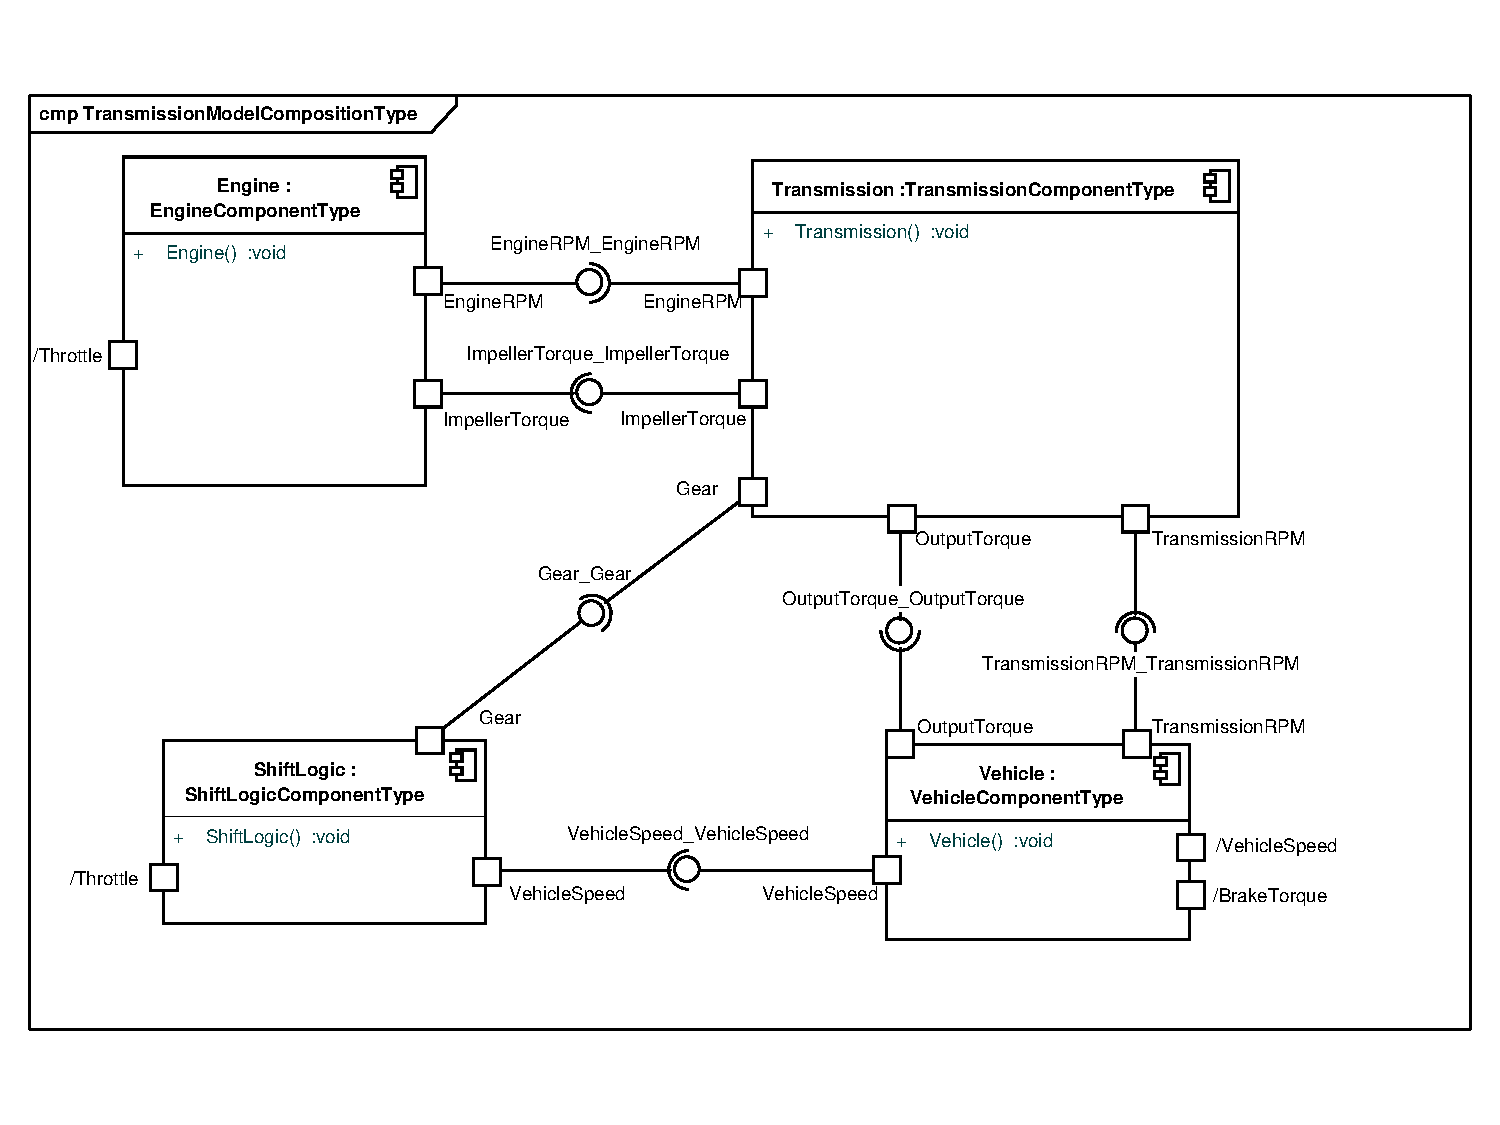
\includegraphics[width=.9\textwidth]{AUTOSARSystem_Componentdiagram}
  \caption{UML component diagram of the system imported to EA}
  \label{fig:autosarsystem}
\end{center}
\end{figure}

\textit{Example:}
The software components in Fig.~\ref{fig:autosarsystem} comply to the blocks of the Simulink model used to generate the implementation of the application code.
This model is used in the MBSecMon development process to describe the allowed and forbidden communication sequences between the components as signatures.   
 
 
\subsubsection{Challenge \ref{itm:datatypesafety}: Providing type safety.}%$~~$\\
In the AUTOSAR development process and in the  automotive domain, specialized data types are used. % to secure data integrity.
This allows for limiting the value range of these data types and prevents wrong assignments such as storing a speed value in a variable intended for the impeller torque.
Generated monitors have to obey this implicit safety mechanism that is inherent in the AUTOSAR standard. 

\textit{MBSecMon process:} 
The special data types provided by the AUTOSAR system specification are imported along with the component diagrams and stored in its ports.  
While modeling the signatures, the developer's choice is constrained to these data types.
These are further used in the monitor generation process and result in type safe monitoring code.

 
\textit{Example:} 
In the ARXML file the data type for the vehicle speed, shown in Listing~\ref{lst:arxmlTypeSafety}, is defined as \emph{VehicleSpeedDataType} with a base type \emph{Double} and is limited to a range of possible values.


\lstset{language=XML,
 basicstyle=\tiny,
 breaklines=true, % Zeilen werden Umgebrochen  
 mathescape=true,
 frame=single,
 captionpos=t,
 showstringspaces=false}
\begin{lstlisting}[float=tb, caption=Type safety in AUTOSAR (ARXML file), label={lst:arxmlTypeSafety}]
<REAL-TYPE >
  <SHORT-NAME>VehicleSpeedDataType</SHORT-NAME>
  <LOWER-LIMIT INTERVAL-TYPE="CLOSED" >-1000.0</LOWER-LIMIT>
  <UPPER-LIMIT INTERVAL-TYPE="CLOSED" >1000.0</UPPER-LIMIT>
  <ALLOW-NAN>false</ALLOW-NAN>
  <ENCODING>DOUBLE</ENCODING>
</REAL-TYPE>
\end{lstlisting}
%\textcolor{red}{Example for datatype definition as xml, it is in ARXML annotated}
  
\subsubsection{Challenge \ref{itm:modelling}: Modeling at the same abstraction level.}%$~~$\\
AUTOSAR system specifications are modeled at a high abstraction level as presented in Challenge~\ref{itm:integrationExisting}.
%describing the  software components (SW-C), their ports with specified data types, and the connections of the ports.
The ports describe which type of communication is used to interact with other SW-Cs over the Virtual Function Bus (VFB).
Thus, it makes sense to monitor the communication between the SW-Cs.
A widespread approach to describe interactions between components are various kinds of sequence charts that are on the same abstraction level as the AUTOSAR specification. 
These descriptions of the interaction between SW-Cs (signatures) can be used to generate monitors.




\begin{figure}[tb]
\begin{center}
  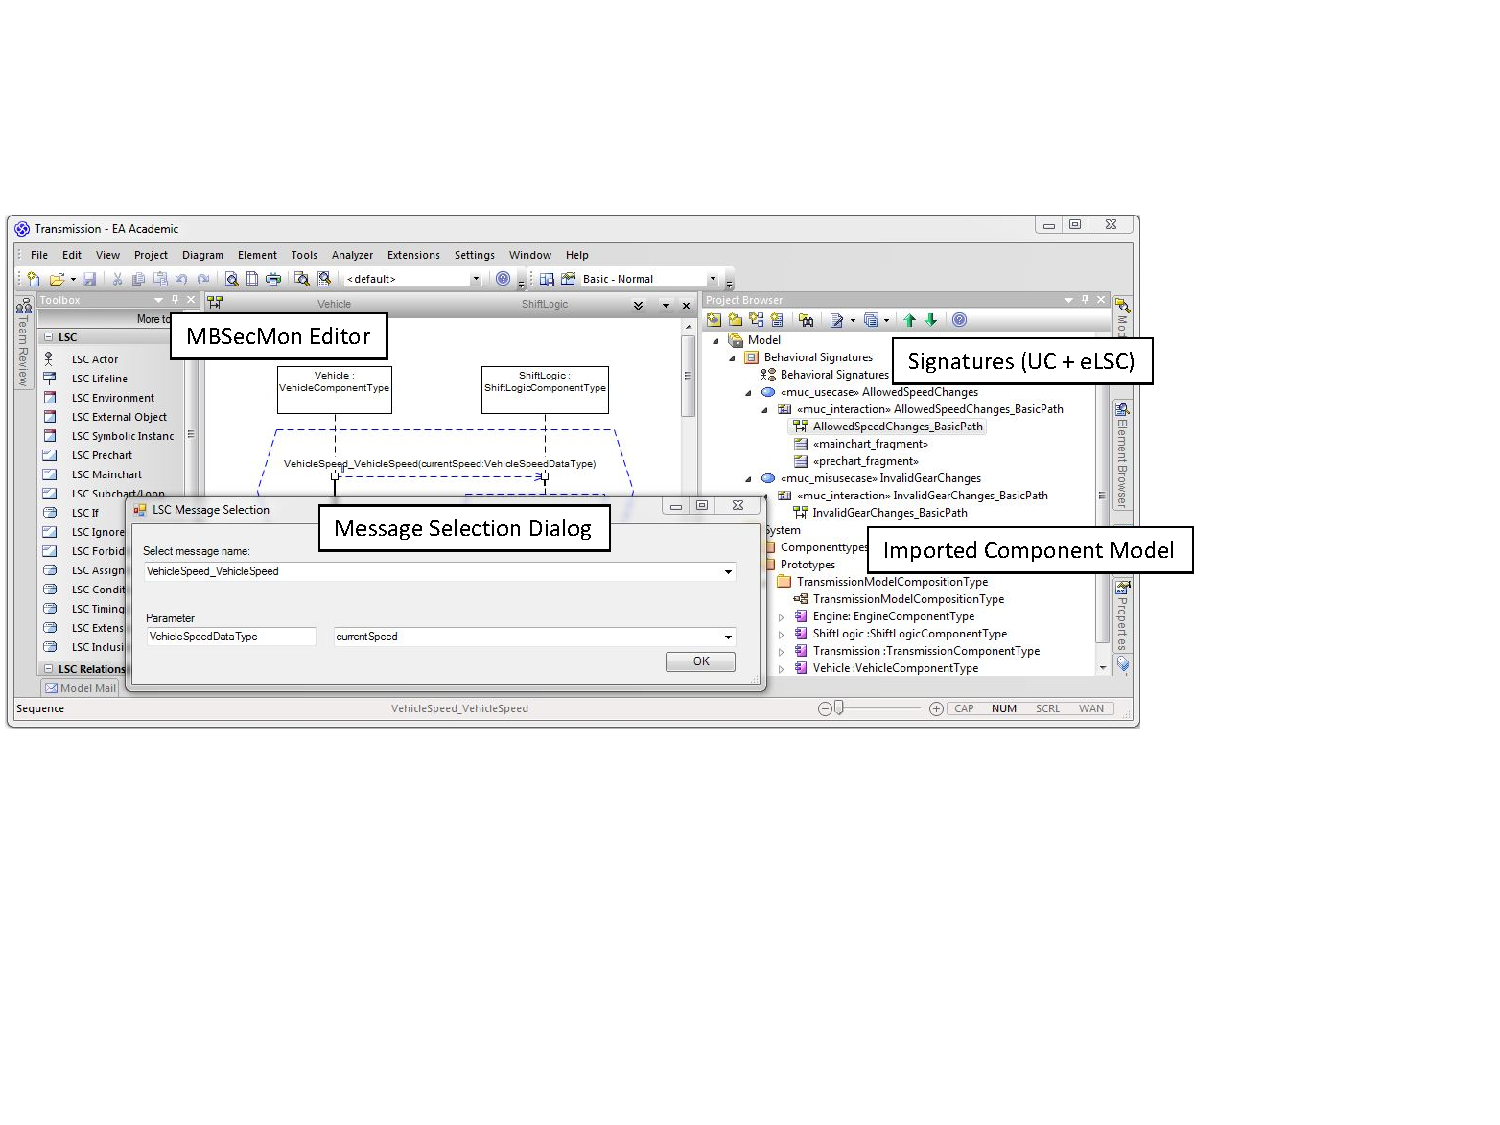
\includegraphics[width=.9\textwidth]{MBSecMonEditor}
  \caption{Tailored Signature Editor for AUTOSAR}
  \label{fig:mbsecmoneditor}
\end{center}
\end{figure}

\textit{MBSecMon process:} 
For this purpose, the MBSecMon specification language (MBSecMonSL), which consists of extended Live Sequence Charts (eLSC) that are structured by use/misuse cases (UC/MUC), is used in the MBSecMon framework.
In addition to the concepts of the wide-spread  Message Sequence Charts~\cite{Harel2004a}, eLSCs distinguish between hot (solid red border) and cold (dashed blue border) elements, where hot elements are mandatory and cold elements are optional.
Furthermore, two forms of eLSCs exist, an universal eLSC with a prechart (precondition) (blue dashed hexagon) before the mainchart (solid black rectangle) and an existential eLSC without a precondition.
In the prechart, every element is interpreted as mandatory.
This is based on the interpretation of the prechart as a precondition.  
When the prechart is fulfilled, the part of the signature in the mainchart is evaluated.

The import of the component view from an AUTOSAR tool to EA forms the basis for the signature modeling.
The MBSecMon EA add-in (Fig.~\ref{fig:mbsecmoneditor}) provides a context sensitive choice of messages between components and their parameter types. 
This ensures the compliance to the modeled AUTOSAR system. 


\begin{figure}[tb]
\begin{center}
  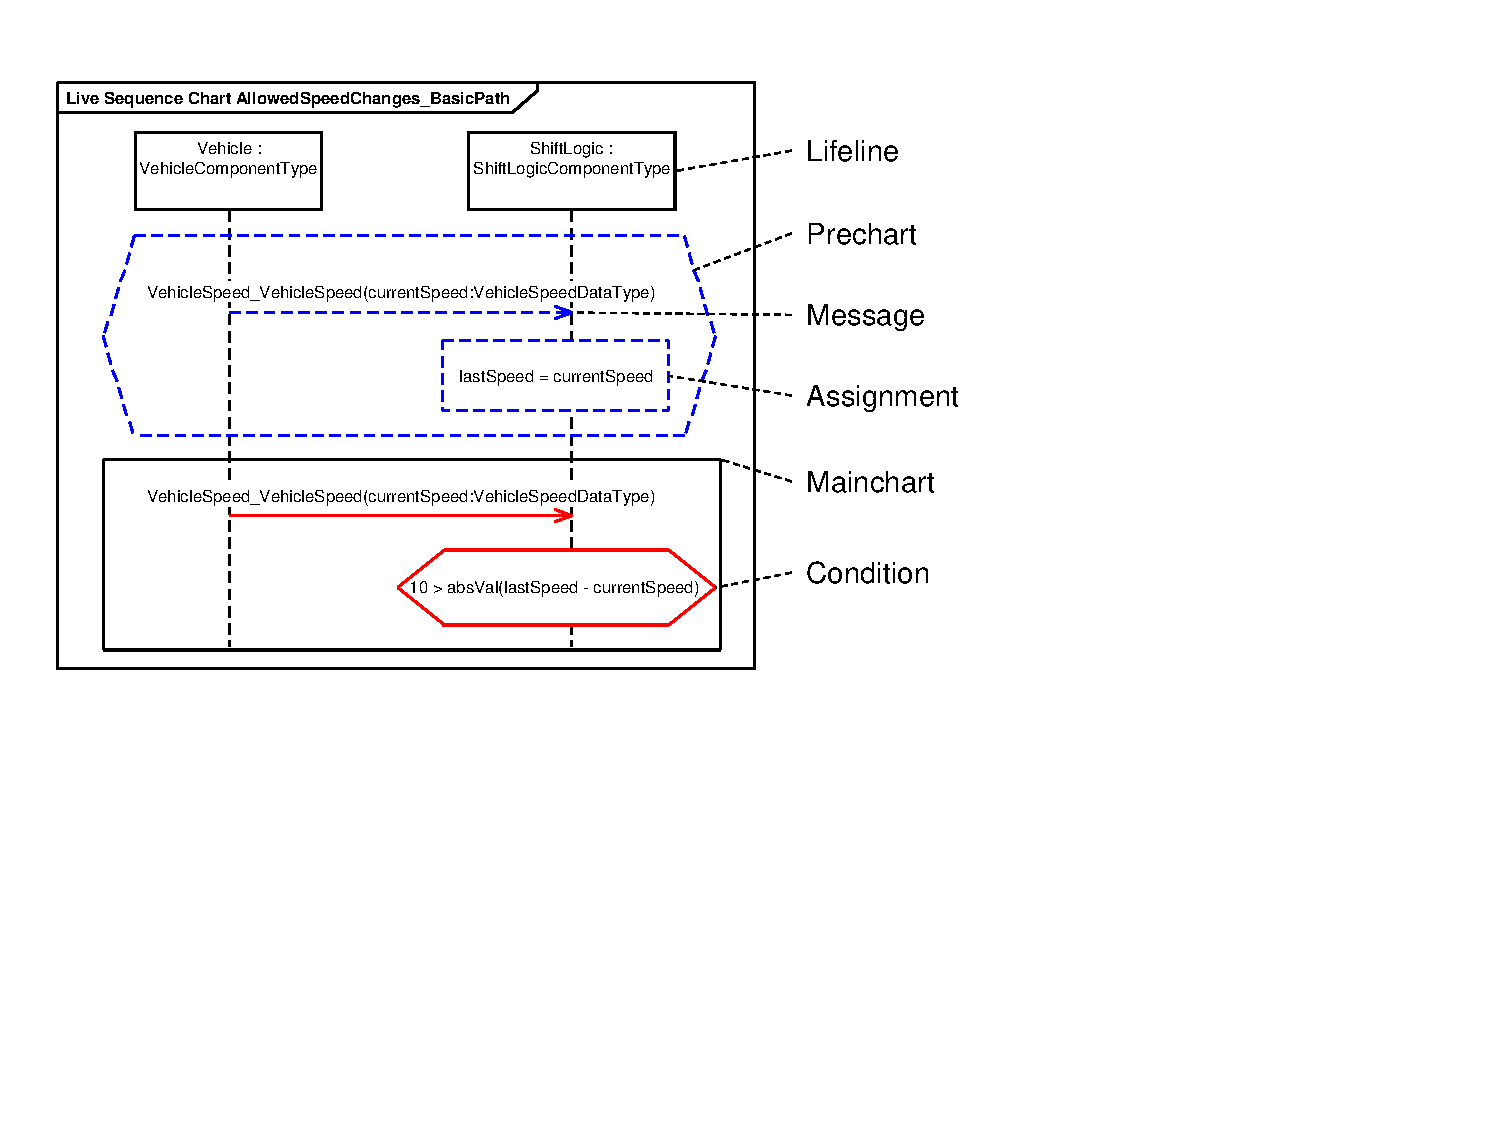
\includegraphics[width=.7\textwidth]{LSCSignatures}
  \caption{Signature of the Use Case ``AllowedSpeedChanges''}
  \label{fig:lscsignatures}
\end{center}
\end{figure}

\textit{Example:} 
Figure~\ref{fig:lscsignatures} shows a simple example of a concurrent signature that uses only the basic elements of the eLSC language.
This signature monitors the communication between the \emph{Vehicle} and the \emph{ShiftLogic} components by initializing the monitor for every message, consisting of a sending and a receiving event, transmitted over the port \emph{VehicleSpeed}.
The message contains the value \emph{currentSpeed} that is stored by the assignment to an eLSC specific variable \emph{lastSpeed}.
The first processed sending event triggers the initialization of a new instance of the signature that concurrently monitors the next messages.
The next \emph{VehicleSpeed} message is processed by the mainchart of the first instance and evaluated by the condition to the previous value stored in \emph{lastSpeed}.
This monitoring instance is then terminated based on the result of the condition. 
Subsequently, the same message is evaluated by the prechart of the second instance of the signature and overwrites the variable \emph{lastSpeed} with the new value. 


\subsubsection{Challenge \ref{itm:mappingsig}: Mapping to platform specific monitoring code.}%$~~$\\
%The signatures modeled in by the MBSecMon EA add-in are exported to a XMI representation based on the MBSecMonSL metamodel~\cite{Patzina2011a} that is used for code generation. 
By modeling signatures on a much more abstract level than the code of the target platform and using an annotation language in the signatures, the code generator needs additional information about the mapping to the target platform. 

\textit{MBSecMon process:} 
To support type safe, AUTOSAR-compliant interfaces for the monitor, additional mappings are generated to the platform specific information (PSI) file. 
It contains mappings between AUTOSAR instrumentation interface and the internal events of the monitor, data types for transferred values, a code mapping of signature annotations to the target domain, and configuration details for the code generation.
Most information for the file can be automatically derived from the imported system specification and the modeled signatures.
Only mappings exported by the EA add-in from annotated pseudo code in the signatures have to be adapted manually to the target language.
For more convenient usage, a mapping library for these annotations could automate this manual step. 

\textit{Example:} 
The generated PSI file provides the mapping of pseudo code used in the signatures to platform-conform code fragments, as depicted in Listing~\ref{lst:lscPSIMapping} for a method \emph{absVal} in the condition of the signature in Fig.~\ref{fig:lscsignatures}.

\lstset{language=XML,
basicstyle=\scriptsize,
mathescape=true,
frame=single,
captionpos=t,
showstringspaces=false}
\begin{lstlisting}[float=tb, caption=LSC specific information in the PSI file, label={lst:lscPSIMapping}]
<entry key="AllowedSpeedChanges_BasicPath.context_method.absVal">fabs
</entry>
\end{lstlisting}

%\textcolor{red}{example for PSI? Example for COHXML?}
%\textcolor{red}{manual changes in PSI file}



\subsubsection{Challenge \ref{itm:connectingmonitors}: Providing communication data to the monitors.}%$~~$\\
The system model of the AUTOSAR specification uses the concept of the Virtual Function Bus (VFB) and only describes the communication pattern (e.g. sender/receiver).
This communication is realized on the target platform depending on the RTE and the allocation of the SW-Cs to the different ECUs.
This hampers the monitoring of the communication between the SW-Cs.

  
\textit{MBSecMon process:}
Based on the signatures, the \emph{instrumenting device} needs a clear naming convention for the monitor interfaces to allow for the wrapping of write and read methods in the AUTOSAR system code. 
Additionally, the \emph{instrumenting device} uses the exported information that specifies, based on the signatures, which ports in the AUTOSAR system have to be instrumented to minimize the footprint of the instrumentation by only adding method calls for the required events.


%The code generation (interfaces and mapping) have been extended to be type save by using the original AUTOSAR data types.
%\textcolor{red}{For code generation, the exported signatures as XMI files are transformed to the intermediate language Monitor Petri nets (MPN).
%This more explicit representation of the signatures are then, together with the platform-specific information, including mappings of events, data types and the replacement of pseudo code, used to generate AUTOSAR conform C code.}

\textit{Example:} 
The interfaces of the monitor are named based on the naming conventions of the AUTOSAR standard.
Thus, the \emph{instrumenting device} can automatically generate calls to the interfaces into the system code.
Listing~\ref{lst:monitorinterfaces} shows the interfaces of the generated example monitor.
The method name is derived by concatenation of the string \texttt{dispatchEvent\_} and the full name of the port of the AUTOSAR component and the data type of the parameter origins from the AUTOSAR model.

\lstset{language=C,
basicstyle=\scriptsize,
mathescape=true,
frame=single,
captionpos=t,
showstringspaces=false}
\begin{lstlisting}[float=tb, caption=Monitor interfaces for the running example, label={lst:monitorinterfaces}]
void dispatchEvent_TransmissionModelCompositionType_Vehicle_
  VehicleSpeed(VehicleSpeedDataType$^*$);
void dispatchEvent_TransmissionModelCompositionType_ShiftLogic_
  VehicleSpeed(VehicleSpeedDataType$^*$);
\end{lstlisting}


%\textcolor{red}{Description of instrumentation concept is missing; with view of paths of two communicating SW-Cs?, instrumentation location, where is the monitor located?}

\subsubsection{Challenge \ref{itm:relocatability}: Supporting the relocatability of software components.} %$~~$\\
One of the important concepts of the AUTOSAR standard is the relocatability of SW-Cs that allows for distributing them to different ECUs without changing the specification.
Due to modeling the monitors on the same abstraction level as the AUTOSAR system specification, the developer of the signatures cannot incorporate information about the final distribution of the SW-Cs.
The code generation process must support the generation of distributed monitors based on the actual distribution of the SW-Cs.
This reduces the run-time overhead for single ECUs and the communication overhead over the buses between the ECUs in contrast to a central monitor.

\textit{MBSecMon process:}
In the MBSecMon generation process, the signatures modeled as eLSCs already contain an affiliation of the events (sending and receiving) to the SW-Cs. 
This affiliation is obtained when the exported signatures are transformed to the intermediate Monitor Petri nets (MPN), and allow for generating distributed monitors based on the SW-C located on the same ECU.
To preserve dependencies between the part monitors (e.g. sending before receiving event of a message), an additional communication between the monitors has to be established.
Therefore, the code generator has been prepared to create identifiers that can be replaced by macro definitions to system communication methods.
          

\textit{Example:} In the example, we use the sender-receiver pattern that directly supports transferability and exchange of AUTOSAR software components.
The two components, \emph{ShiftLogic} and \emph{Vehicle}, in the signature in Fig.~\ref{fig:lscsignatures} can be distributed to different ECUs by defining ``\lstset{basicstyle=\normalsize}\lstinline{ShiftLogic;$\{$Vehicle$\}$}'' in the PSI file the instance that is on the same ECU (\emph{ShiftLogic}) and the instances (\emph{Vehicle}) that is located on another ECU and should be synchronized with it. 

  

\subsubsection{Challenge \ref{itm:minimalOverhead}: Generating monitors with a minimal overhead.} %$~~$\\
The generated run-time monitors are deployed on the ECUs and run alongside the SW-Cs.
Hence, their induced run-time and memory overhead on the ECUs have to be sufficiently small.
The reasonable overhead depends on the required level of safety and security that has to be reached by monitoring.
For the runtime-overhead, a worst case upper bound can be calculated by a static analysis of the signatures in the MPN format.

\textit{Example:} In the presented example in Figure~\ref{fig:lscsignatures} the monitor has to evaluate two transitions per monitor instance (sending or receiving events) in one event processing step.
Additionally, to this computation the annotated assignment or condition has to be taken into account.   

%Hence, they can only add a run-time and memory overhead to the ECUs that is sufficiently small.      
The evaluation in Sect.~\ref{sec:evaluation} shows the overhead that the resulting monitors introduce to the system.






\section{Evaluation}
\label{sec:evaluation}
For the evaluation of the MBSecMon specification and generation process for AUTOSAR, an adaptation of the Simulink example model \emph{Automatic Transmission Controller}~\cite{TheMathWorks2012}, as presented in Sect.~\ref{sec:example}, is used.
In order to provide compatibility with Simulink's AUTOSAR code generator, which does not support the continuous blocks (such as integrators) that were used in the original example, we decomposed the example model into separate software components and replaced the incompatible blocks with their corresponding discrete versions.
The generated code contains the runnables (executable entities) of each software component (SW-C), which have to be integrated into the implementation code skeleton that was generated by the system level design and simulation tool OptXware Embedded Architect (OXEA).
In OXEA, we have also designed the system model that corresponds to the Simulink example, and which is stored in the standardized ARXML format.

We instrumented the evaluation system with two different monitors (cf. Fig.~\ref{fig:simulinkExample}).
The first one is \emph{AllowedSpeedChanges}, as presented in Sect.~\ref{sec:mbsecmonFramework}, which monitors the communication between the components \emph{Vehicle} and \emph{ShiftLogic} in order to detect a communication error between these components.
The monitor signals an error in case that it detects a difference between two consecutive speed readings that is larger than 10\,mph within a 20\,ms timeframe (the period of the tasks).
The second one is \emph{InvalidGearChanges}, which, in contrast to the first signature, monitors the misuse case of a gear shifting by more than one step within a 20\,ms timeframe. Therefore, the communication between the components \emph{ShiftLogic} and \emph{Transmission} is monitored.
Based on these two signatures, a monitor that consists of a controller and a monitor representation for each signature is generated by the MBSecMon process.

The evaluation covers the run-time overhead that the monitoring induces per instrumented port (\emph{Gear} for ShiftLogic and Transmission, and \emph{VehicleSpeed} for Vehicle and ShiftLogic), and per instrumented runnable (Vehicle, ShiftLogic, Transmission).
Furthermore, we analyze the memory overhead of the monitors, for both, code and data segments.
Finally, a scalability analysis on an embedded system is performed.

% Additionally to the signature \emph{AllowedSpeedChanges} presented in Sect.~\ref{sec:mbsecmonFramework}, a second signature \emph{InvalidGearChanges} is added. 
% In contrast to the first, this signature describes a misuse case, where a gear shift of more than one step at once is detected.
% Based on these two signatures, a monitor that consists of a controller and a monitor representation for each signature is generated by the MBSecMon process. 

\subsubsection{Run-time analysis.} The evaluation was conducted using OptXware EA's simulation environment on a AMD Phenom II X4 955 processor, running at 3.20\,GHz.
The timing measurements were taken using the Win32 API functions \emph{MyQueryPerformanceCounter} and \emph{MyQueryPerformanceFrequency}, which are Window's high resolution timing functions, providing CPU tick granularity.
This is a best effort solution, as there is no commonly agreed on reference architecture for such evaluation.
Therefore, we also provide relative measurements of the execution time overhead as comparison.

Figure~\ref{fig:simulationInput} shows the input data (readings of the throttle and brake torque sensor) for the test run of the automatic transmission model.
It represents a passing maneuver, where the vehicle approaches a slower car and then abruptly accelerates to pass the car.

\begin{figure}[tb]
\centering
\subfloat{
\pgfplotstableread{sections/PassingManeuver.dat}{\pistonkinetics}
\begin{tikzpicture}[scale=0.6]
\begin{axis}[xlabel={Time in s},  scaled x ticks = false, ylabel={Throttle in $\%$}, height=4cm, width=9cm, ymin=-5, ymax=110]
\addplot [black,very thick] table [x=time, y=throttle, col sep=semicolon] {sections/PassingManeuver.dat};
\end{axis}
\end{tikzpicture}
}
\qquad
\subfloat{
\begin{tikzpicture}[scale=0.6]
\begin{axis}[xlabel={Time in s}, ylabel={Brake torque in $\%$}, height=4cm, width=9cm, , ymin=-5, ymax=110]
\addplot [black,very thick] table [x=time, y=break, col sep=semicolon] {sections/PassingManeuver.dat};
\end{axis}
\end{tikzpicture}
}

\caption{Input data set for the passing maneuver}
\label{fig:simulationInput}
\end{figure}


% \begin{figure}[htp]
% \begin{center}
%   \includegraphics[width=.6\textwidth]{SimulationInput.jpg}
%   \caption{Passing Maneuver}
%   \label{fig:simulationInput}
% \end{center}
% \end{figure}

Table~\ref{tab:resultsO0RteCall} shows the run-time for performing calls to the RTE in the simulation environment without (\emph{Original}) and with instrumentation (\emph{Instr.}).
The measured time for the instrumented RTE calls includes the wrapper around the call method, the invocation of the monitor, and the evaluation of the event by the monitor.
The overhead is between 28 and 31\% for write calls and between 49 and 57\% for read calls.
This difference results from the structure of the signatures that include an additional assignment or condition in the monitor for the transmitted value at the receiving side (read call).



\begin{table}[tb]
\centering\setlength{\tabcolsep}{3pt}
\scriptsize
 \caption{Execution time comparison of original and monitored calls to the RTE}
 \begin{tabular}{llccc}\toprule
 &  & \multicolumn{2}{c}{\textbf{Average}}&\\
 \textbf{Component}&\textbf{RTE Call}  & \emph{Original} \emph{(ticks)} & \emph{Instr. (ticks)} & \emph{Diff. ($\%$)}\\
% $\begin{array}{l} \mbox{\emph{Original}}\\\mbox{\emph{(ticks)}}\end{array}$ & $\begin{array}{l} \mbox{\emph{Instr.}}\\\mbox{\emph{(ticks)}}\end{array}$ & $\begin{array}{l} \mbox{\emph{Diff.}}\\\mbox{\emph{($\%$)}}\end{array}$\\
 \cmidrule(r){1-2}\cmidrule(r){3-4}\cmidrule(r){5-5}
ShiftLogic() & Rte\_Read\_VehicleSpeed \ldots 	& 24,76 & 38,87 &57\\
ShiftLogic() & Rte\_Write\_Gear \ldots 		& 18,00 & 23,60 &31\\
Transmission() & Rte\_Read\_Gear \ldots 		& 25,28 & 37,63 &49\\
Vehicle() & Rte\_Write\_VehicleSpeed \ldots 	& 21,56 & 27,62 &28\\\bottomrule
 \end{tabular}
 \label{tab:resultsO0RteCall}
\end{table}


Table~\ref{tab:resultsO0Runnable} shows the influence of the monitor on the total run-time of the \mbox{SW-C's} runnables.
For the ShiftLogic component, two ports have been wrapped and, therefore, the instrumented runnable calls the monitor twice as often as for the other components.
The components Transmission and Vehicle, which contain only one instrumented port, therefore, have a smaller run-time overhead.
%Despite the two monitor signatures having comparable complexity, the run-time overhead differs.
%This results from the optimizations done by the C code compiler, that only works for the Transmission component.
%\TODO{\ldots optimierter Code entspricht nicht Erwartung und tabelle \ref{tab:resultsO0RteCall}} 
%Halte ich f�r einen Leser der die Interna nicht kennt f�r schwer nachvollziehbar. W�rde es daher, um Verwirrung zu vermeiden, eher rauslassen.
\begin{table}[tb]
\centering\setlength{\tabcolsep}{4pt}
\scriptsize
 \caption{Execution time comparison of original and monitored runnables}
 \begin{tabular}{lcccc}\toprule
 &   \multicolumn{2}{c}{\textbf{Average}}&&\\
\textbf{Component} & \emph{Original (ticks)} & \emph{Instr. (ticks)} & \emph{Diff. (ticks)}& \emph{Diff. ($\%$)}\\   
%$\begin{array}{l} \mbox{\emph{Original}}\\\mbox{\emph{(ticks)}}\end{array}$ & $\begin{array}{l} \mbox{\emph{Instr.}}\\\mbox{\emph{(ticks)}}\end{array}$ & $\begin{array}{l} \mbox{\emph{Diff.}}\\\mbox{\emph{(ticks)}}\end{array}$&$\begin{array}{l} \mbox{\emph{Diff.}}\\\mbox{\emph{($\%$)}}\end{array}$\\
\cmidrule(r){1-1}\cmidrule(r){2-3}\cmidrule(r){4-5}
ShiftLogic()  	& 56,03 & 70,97	&14,94&28\\
Transmission()  & 57,28 & 63,77	&6,49&11\\
Vehicle() 		& 48,63 & 58,39 &9,76&20\\\bottomrule
 \end{tabular}
 \label{tab:resultsO0Runnable}
\end{table}

\subsubsection{Memory overhead.} We conducted our analysis of the memory overhead using the tool \emph{objdump} of the GNU binutils toolsuite on the compiled object files.
\mbox{Objdump} provides a detailed overview of the memory consumption of the text (aka. code) section, and the three data sections data, bss (uninitialized data) and rdata (read-only data).
The analysis of the memory overhead of the integrated monitors is depicted in Tab.~\ref{tab:memoryOverhead}.
The first four columns show the memory that is consumed by the RTE call wrappers that pass the signals to the monitor.
As the functionality of each wrapper is similar, their overhead is constant.

The monitor component consists of a controller (\emph{Contr.}) that manages the monitors and the signatures AllowedSpeedChanges (\emph{ASC}) and InvalidGearChan\-ges (\emph{IGC}).
The controller caches the transmitted values, triggers the signature representations, and evaluates their results.
%Das ist so nicht korrekt. In AUTOSAR gibt es keinen dynamischen Speicher. Sollten dennoch irgendwelche Aufrufe zu zB malloc() vorhanden sein w�re das ganze auf einem echten AUTOSAR System nicht lauff�hig!
%Wir sollten die Darstellungsweise der Data-Section nochmal �berdenken; die Bedeutung der Zahlen in Klammern ist nicht erkl�rt.
%Will das ungern ohne R�cksprache mit euch entscheiden, daher lass ich es erstmal so.
The memory overhead of the data section is very small and grows very slowly with the complexity of the signatures because only the state of the monitor and the monitor specific variables, as shown in Sect.~\ref{sec:example}, are stored there.
%As stated at the evaluation of the run-time, the signatures differ in their execution time caused by the optimisation of the C compiler.
%This is also reflected in the code size.
%The signature \emph{ASC}, whose execution time is smaller, has a higher static memory foot print.  
%obige 3 zeilen sind nicht zutreffend

\begin{table}[tb]
\centering\setlength{\tabcolsep}{4pt}
\scriptsize
\caption{Memory overhead caused by the monitors in byte}
 \begin{tabular}{lccccccc}\toprule
 &   \multicolumn{4}{c}{\textbf{Wrapper}}&\multicolumn{3}{c}{\textbf{Monitor}}\\
\textbf{Type} &   \emph{Read\_VS} &\emph{Write\_VS} &\emph{Read\_G} & \emph{Write\_G}&\emph{Contr.}&\emph{ASC}&\emph{IGC}\\\cmidrule(r){1-1}\cmidrule(r){2-5}\cmidrule(r){6-8}
Code  & 48	& 48	& 48	& 48 	& 1632 	& 2512	& 2160\\
Data  & 0 	& 0 	& 0 	& 0		& 88 	& 40 	& 32 \\\bottomrule
% Data  & 0 	& 0 	& 0 	& 0		& 88 (92) 	& 30 (336)	& 30 (240)\\\bottomrule
 \end{tabular}
 
 \label{tab:memoryOverhead}
\end{table}


\subsubsection{Scalability analysis.} The previous results have shown that the generated monitors can be used in an AUTOSAR environment with reasonable overhead. 
For the evaluation of the scalability of the monitors, various models of different complexity are generated and the run-time behaviour of the generated C code is measured on a Fujitsu SK-16FX-100PMC evaluation board equipped with an F$^2$MC-16FX MB96340 series microcontroller (16\,bit, 56\,MHz).
Table~\ref{tab:evaluation} shows the different models, the run-time of the generated monitors for processing one event in the signature, where a message  consists of a sending and receiving event, and the needed memory on the micro controller.
The values for the needed data memory (RAM) include approximately 800 bytes of data that do not origin from the generated monitor.
For the measurement of the run-time, 1000 complete runs of the signatures have been performed.
Complex conditions and actions in the signature are dismissed and only the monitor itself is measured. 

\begin{table}[tb]
\begin{center}
\setlength{\tabcolsep}{3.5pt}
\scriptsize
\caption{Results of the scalability evaluation}
\begin{tabular}{@{}llrrrr@{}}
\toprule
\textit{Model} &\textit{\#Messages} &\textit{Different} \textit{events}&  \textit{Run-time/}\textit{Event in} $\mu s$ & \textit{Code} \textit{in byte}& \textit{Data} \textit{in byte} \\
\cmidrule(){1-1}\cmidrule(lr){2-2}\cmidrule(lr){3-3}\cmidrule(lr){4-4}\cmidrule(lr){5-5}\cmidrule(){6-6}
 M1 &  1  & 2            & 28,384 &896 & 1038\\
 M2 &  2  & 4            & 25,360 &1078 &1044\\
 M3 &  3  & 6            & 24,277  &1230 &1044\\
 M4 &  4 &  8            & 23,728  &1382 &1044\\
 M5 &  50  & 100       & 22,636 & 8898&1154\\     
 M6 &  100  & 200       & 22,660  & 17026&1268\\
 M7 & 	2  & 2           & 25,936  &1043 &1044\\
 M8 & 	3  & 2           & 25,099  &1158 &1044\\
 M9& 	4  & 2           & 25,176  &1562 &1044\\
 M10&  50  & 2         &  46,239 & 7260&1156\\
 M11&  100  & 2         &  67,973 & 13605&1270\\
 M12&  2 * M4 & 8   & 46,424  &2696 &1056\\
 M13&  3 * M4 & 8   & 67,992   &4000 &1068\\
 M14& 4 * M4 & 8   & 89,744  & 5304&1080\\
\bottomrule
\end{tabular}
\label{tab:evaluation}
\end{center}
\end{table}

Model 1 to 6 demonstrate how the monitors scale if the number of messages increases in the signature. 
Model 1 and 7 to 11 show the overhead when all messages have the same message type.
In Model 4 and 12 to 14, the number of signatures of constant size (M4) is increased.
With an increasing number of processing steps to reach the final state of the signature the initialization overhead gets less important. 
The code memory consumption increases linearly with the number of messages located in a signature.
In all cases, the RAM needed to store the state of the signature increases very slowly, because the state of the signature is binary coded.
This is an important factor for use on resource constrained embedded systems.
The evaluation shows that the monitors have a constant computing time per processed event (M1 to M6) and only a linear increase for processing an event that is annotated at multiple transitions (M1, M7 to M11). 


% used instrumentation method and why
% fault injection
% \begin{itemize}
%   \item Overhead: Memory and run-time, maybe SLOC
%   \item SWIFI experiment for validation of the monitor
%   \item Overhead of the monitor/instrumentation\cite{Piper2012}
% \end{itemize}
% 
% 
% Conclusions of the evaluation:
% \begin{itemize}
%   \item low overhead (monitor and instrumentation), is usable on embedded systems
%   \item Errors due to integration of system information into modeling process not likely
%   \item What is with the modeling?
%   \item The overhead of the monitoring code has to be considered in the scheduling.
%   \item Possibility to monitor black box components, because only communication between components is regarded 
%   \item \ldots
% \end{itemize}
\section{Conclusion and Future Work}\label{sec:conclusion}
In this paper, we have identified and addressed the challenges that emerge from integrating run-time monitoring of complex signatures into the AUTOSAR development process.
The presented continuous model-based development process for security and safety monitors (MBSecMon) is integrated into the AUTOSAR process and incorporates data of the AUTOSAR models.
As shown, it allows the modeling of monitor signatures in a well comprehensible graphical modeling language and the automatic generation of monitors with a low overhead that fulfill the AUTOSAR conventions.
This framework and the generated monitors have been evaluated utilizing an example model provided with the MATLAB suite, for which AUTOSAR code was generated and integrated into an AUTOSAR environment.
With the presented approach, we have overcome the lack of support for complex monitoring in the AUTOSAR tool chains.
It is applicable to white-box (source code) and black-box (binary) components, as communication between components is intercepted directly at their port interface by instrumentation techniques shown in~\cite{Piper2012}.

In the future, an evaluation in a larger AUTOSAR project with more complex interactions is planned.
% Find ich eher verwirrend als Leser, der von den verschiedenen Kommunikationsparadigmen in AUTOSAR keine Ahnung hat.
%Additionally, the prototypical implementation can be extended to support the client-server communication of the Virtual Functional Bus between the SW-Cs. 
It has to be evaluated if the MBSecMon process can be used for Logical Program Flow Monitoring~\cite{AUTOSAR_WDM_SPEC}, eventually with another source specification language such as UML2 activity diagrams or MPNs directly. 
% use section* for acknowledgement
\subsubsection*{Acknowledgements.}
This work was supported by CASED (www.cased.de).

\bibliographystyle{template/splncs03}
\bibliography{ECMFA2013}

%\end{linenumbers}
\end{document}
